\setauthor{Arwed Schnalzenberger}

\section{Architekturdiagramm}

\begin{figure} [h t]
    \centering
    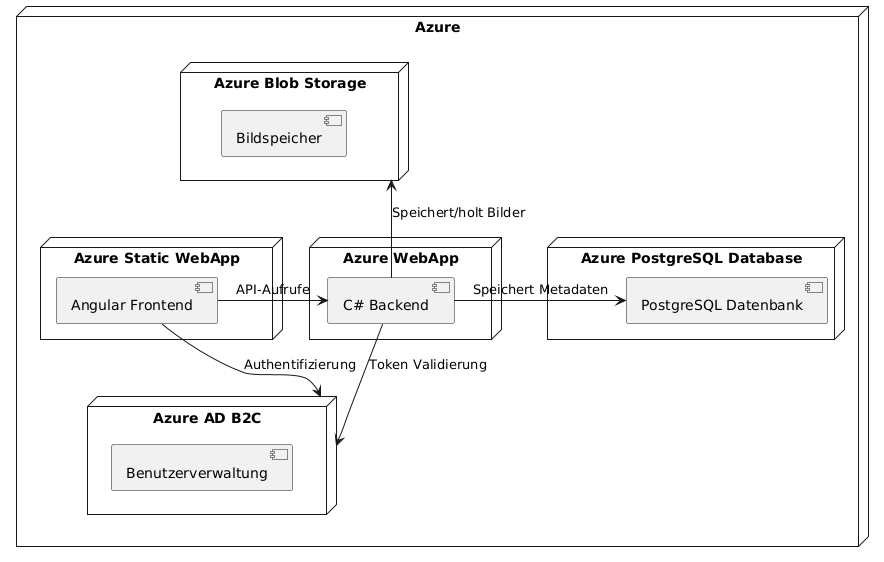
\includegraphics[scale=0.4]{puml/architecture-diagram.png}
    \caption{Architekturdiagramm}
    \label{fig:architectur-diagram}
\end{figure}

Das oben stehende Diagramm \ref{fig:architectur-diagram} zeigt die Architektur von Memoryland,
welches auf der Azure Cloud läuft. Hierbei gibt es mehrere Bestandteile, 
einschlie\ss{}lich eines Frontends, eines C\# Backends, einer Benutzerverwaltung 
über Azure AD B2C und abschlie\ss{}end einer PostgreSQL-Datenbank und einem 
Blob-Storage für die Datenhaltung.

\section{Datenhaltung}

In unserer Datenverwaltung kommen zwei Hauptkomponenten zum Einsatz, welche sich um die 
Speicherung und Verwaltung der Bilddaten kümmern. Ein Azure Blob Storage und eine Azure 
PostgreSQL Datenbank.

\subsection{Azure Blob Storage}

Hier werden die Bilder der Benutzer:innen gespeichert. Diese werden 
ohne eine Struktur abgelegt, au\ss{}er dass für jede/n Benutzer:in ein separater Container erstellt 
wird. Somit wird der kostenpflichtige Zugriff auf den Blob Storage minimiert und die Verwaltung
so einfach wie möglich gehalten.
\footnote{Mehr Info dazu im Kapitel: \ref{subsection:azure_blob_storage_datamodel}}
\footnote{Was ist \emph{Azure Blob Storage} und warum verwenden wir es: Kapitel \ref{subsection:azure_blob_storage}}

\subsection{Azure PostgreSQL Datenbank}

Diese Datenbank speichert die Metadaten zu den Bildern. 
Sie hält zum Beispiel Informationen darüber, in welchen Alben sich welche Erinnerungen befinden
und wem sie gehören neben anderen Details. Zusätzlich verwaltet die PostgreSQL-Datenbank die 
Struktur der Memorylands. Hier stehen unter anderem Informationen, welches Bild zu welchem 
Memoryland gehört, und wo diese im Memoryland platziert werden soll.
\footnote{Mehr Info dazu im Kapitel: \ref{chapter:datamodel}}
\footnote{Was ist \emph{Azure PostgreSQL Datenbank} und warum verwenden wir es: Kapitel \ref{subsection:postgres_db}}

\section{Benutzerverwaltung}

Die Benutzerverwaltung erfolgt über Azure AD B2C. Die Benutzer:innen authentifizieren sich 
im Frontend mithilfe von MSAL (Microsoft Authentication Library), während das Backend 
ihre Berechtigungen gegen Azure AD B2C überprüft.
\footnote{Mehr Info zu Azure AD B2C im Kapitel: \ref{subsection:azure_ad_b2c}}
\footnote{Mehr Info zu MSAL im Kapitel: \ref{subsection:azure_ad_b2c}}

\section{Backend}

Das Backend dient dazu, die Daten von Benutzern:innen mit den erforderlichen
Berechtigungen, zu verwalten. Zu diesen Daten gehören unter anderem Memorylands, 
Alben und Bilder. \footnote{Mehr Info dazu im Kapitel: \ref{chapter:backend-implementation}}

\section{Frontend}

Das Frontend dient als Schnittstelle zum:r Benutzer:in und bietet eine grafische 
Oberfläche zur Verwaltung ihrer Daten. Zudem ermöglicht es eine Darstellung 
der gespeicherten Bilder und Memorylands.
\footnote{Mehr Info dazu im Kapitel: \ref{chapter:frontend-implementation}}

